%!TEX root = main.tex
\chapter{Background}

\section{Computer supported reflection}
Reflection is critical to workplace learning, enabling employees to make sense of complex and dynamic situations\cite{Schon1983}. Boud et al.\cite{boudreflection1985} defined learning through reflection as \emph{those intellectual and affective activities in which individuals engage to explore their experiences in order to lead to new understandings and appreciations.}
The MIRROR project\footnote{\url{http://www.mirror-project.eu/}}, describes reflective learning as the \emph{conscious re-evaluation of experience for the purpose of guiding future behavior, acknowledging the need to attend to feelings, ideas as well as behavior associated with work experience.}\cite{krogstiemodel}.\\*
Work and reflection on this work are heavily connected\cite{Schon1983}, both driving each other forward. Experiences are created through work, and these experiences can be reflected upon. Reflection can be based on both a memory of an experience, and on data from the experience. Revisiting and reflecting on a work experience leads to a better understanding of the experience and allows for learning from it. Reflection can help developers learn from experiences and gain knowledge of how to deal with work-related challenges. This relationship between reflection and learning has been modeled as an experience-based learning cycle\cite{boudreflection1985,Korthagen_Vasalos_2005, KolbModel}. In the reflective process you return to the experience, attend to connected feelings and re-evaluate
the experience. These cycles show that the reflective process and the experience connects in order to produce an outcome. This result with identified behavioural changes and new perspectives. 
Reflection has both individual and social dimensions,\cite{Høyrup_2004,Woerkom_Croon_2008}. Social wise reflection is often performed collaboratively by teams performing a joint task as organised practice, and therefore shares some common ground and experience. \\*
Most reflective learning in a work environment, happens analogically without support of technology\cite{Schindler_Eppler_2003}. Technology has been shown to increase the potency of reflection and reflective learning at work, computer-supported reflection tools can be used developed to promote reflection and experience based learning\cite{krogstiereflectionwork, Lin_Hmelo_Kinzer_Secules_1999,Xiao_Clark_Rosson_Carroll_2008}. 

\subsection{The MIRROR model}
\label{mirrorsection}
The MIRROR model off Computer Supported Reflective Learning (CSRL), is a work on how to incorporate reflection in to the daily routine at work.
MIRROR presents a reflection-learning cycle based on\ref{csrlmodel} which is shown in \ref{mirrormodel}. One key part of this model is the reflection session. These sessions is where the team gathers and actively reflects on experiences, both informal or formal. The model shows that the reflective process and the experience connects in order to produce an outcome. This result with identified behavioural changes and new perspectives can then be applied to the working environment. 
\begin{figure}[!htpb]
\label{csrlmodel}
\centering
	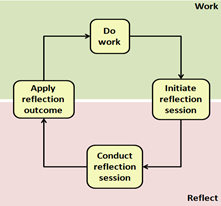
\includegraphics[width=0.8\textwidth]{csrlmodel}
\caption{CSRL Cycle view}
\end{figure}

\begin{figure}[!htpb]
\label{mirrormodel}
\centering
	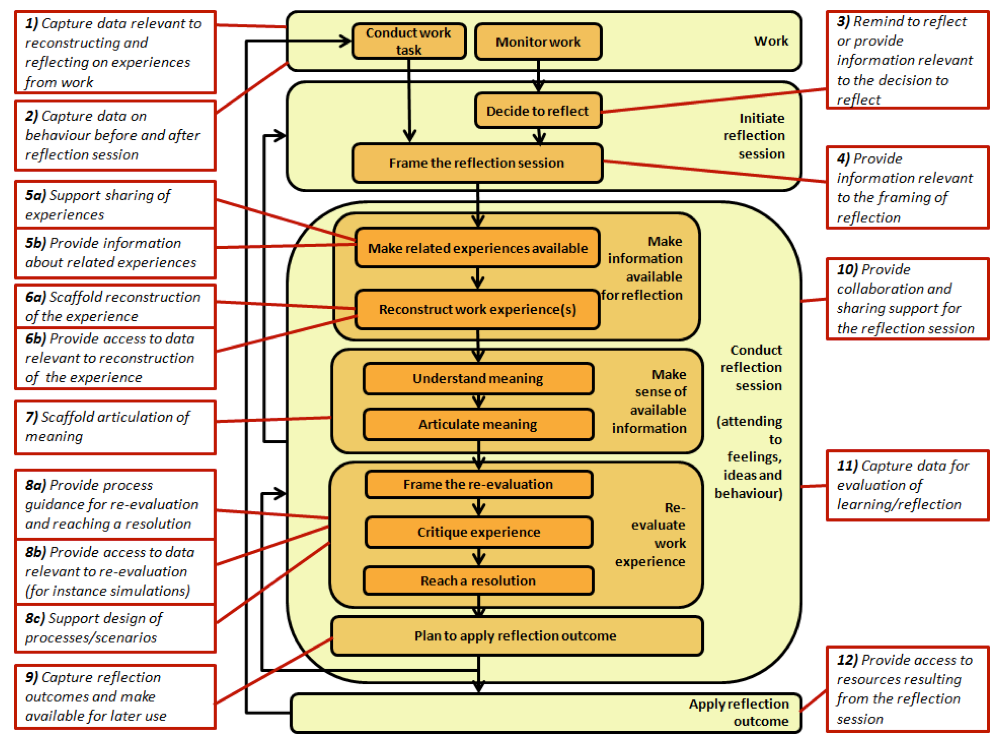
\includegraphics[width=0.8\textwidth]{mirror}
\caption{MIRROR model}
\end{figure}

% Les gjennom dette kapitlet et par ganger. Er nok noen setninger som bør skrives om.
% TODO: Skrive mer om mirror modellen og hvilke steg som er viktige kanskje? DUnno om dette kanskje bør komme senere evt. 

In this thesis, we will utilize this model during the development of the proof-of-concept prototype. This prototype will capture experiences and store them for use in reflection sessions. This will make it easy for users to revisit the experience and reflect upon them, be it individually or collaboratively with a team. The challenge will be to apply the correct steps in order to collect the most important information for the different contexts, and discard the less important data. This is vital in order for our tool to collect the behaviour, ideas and feelings connected to the experience, in order to revisit and reflect upon it. 


%\subsection{Birgits PHD}
% PhD: http://www.idi.ntnu.no/research/doctor_theses/birgitkr.pdf  .

\section{Agile Software Development}
Theoretical background about agile development. Normaly a project is divided into milestones, these milestones will then again be divided into issues and weighted on how much work is required to finish working on each of them.\linebreak
\emph{Manifesto for Agile Software Development:}\cite{agilemanifesto}
\begin{quotation}
We are uncovering better ways of developing software by doing it and helping others do it. Through this work we have come to value:
\begin{itemize}
\item Individuals and interactions over processes and tools
\item Working software over comprehensive documentation
\item Customer collaboration over contract negotiation
\item Responding to change over following a plan
\end{itemize}
That is, while there is value in the items on
the right, we value the items on the left more.\\*
\end{quotation}

\begin{figure}[!htpb]
\label{logo}
\centering
	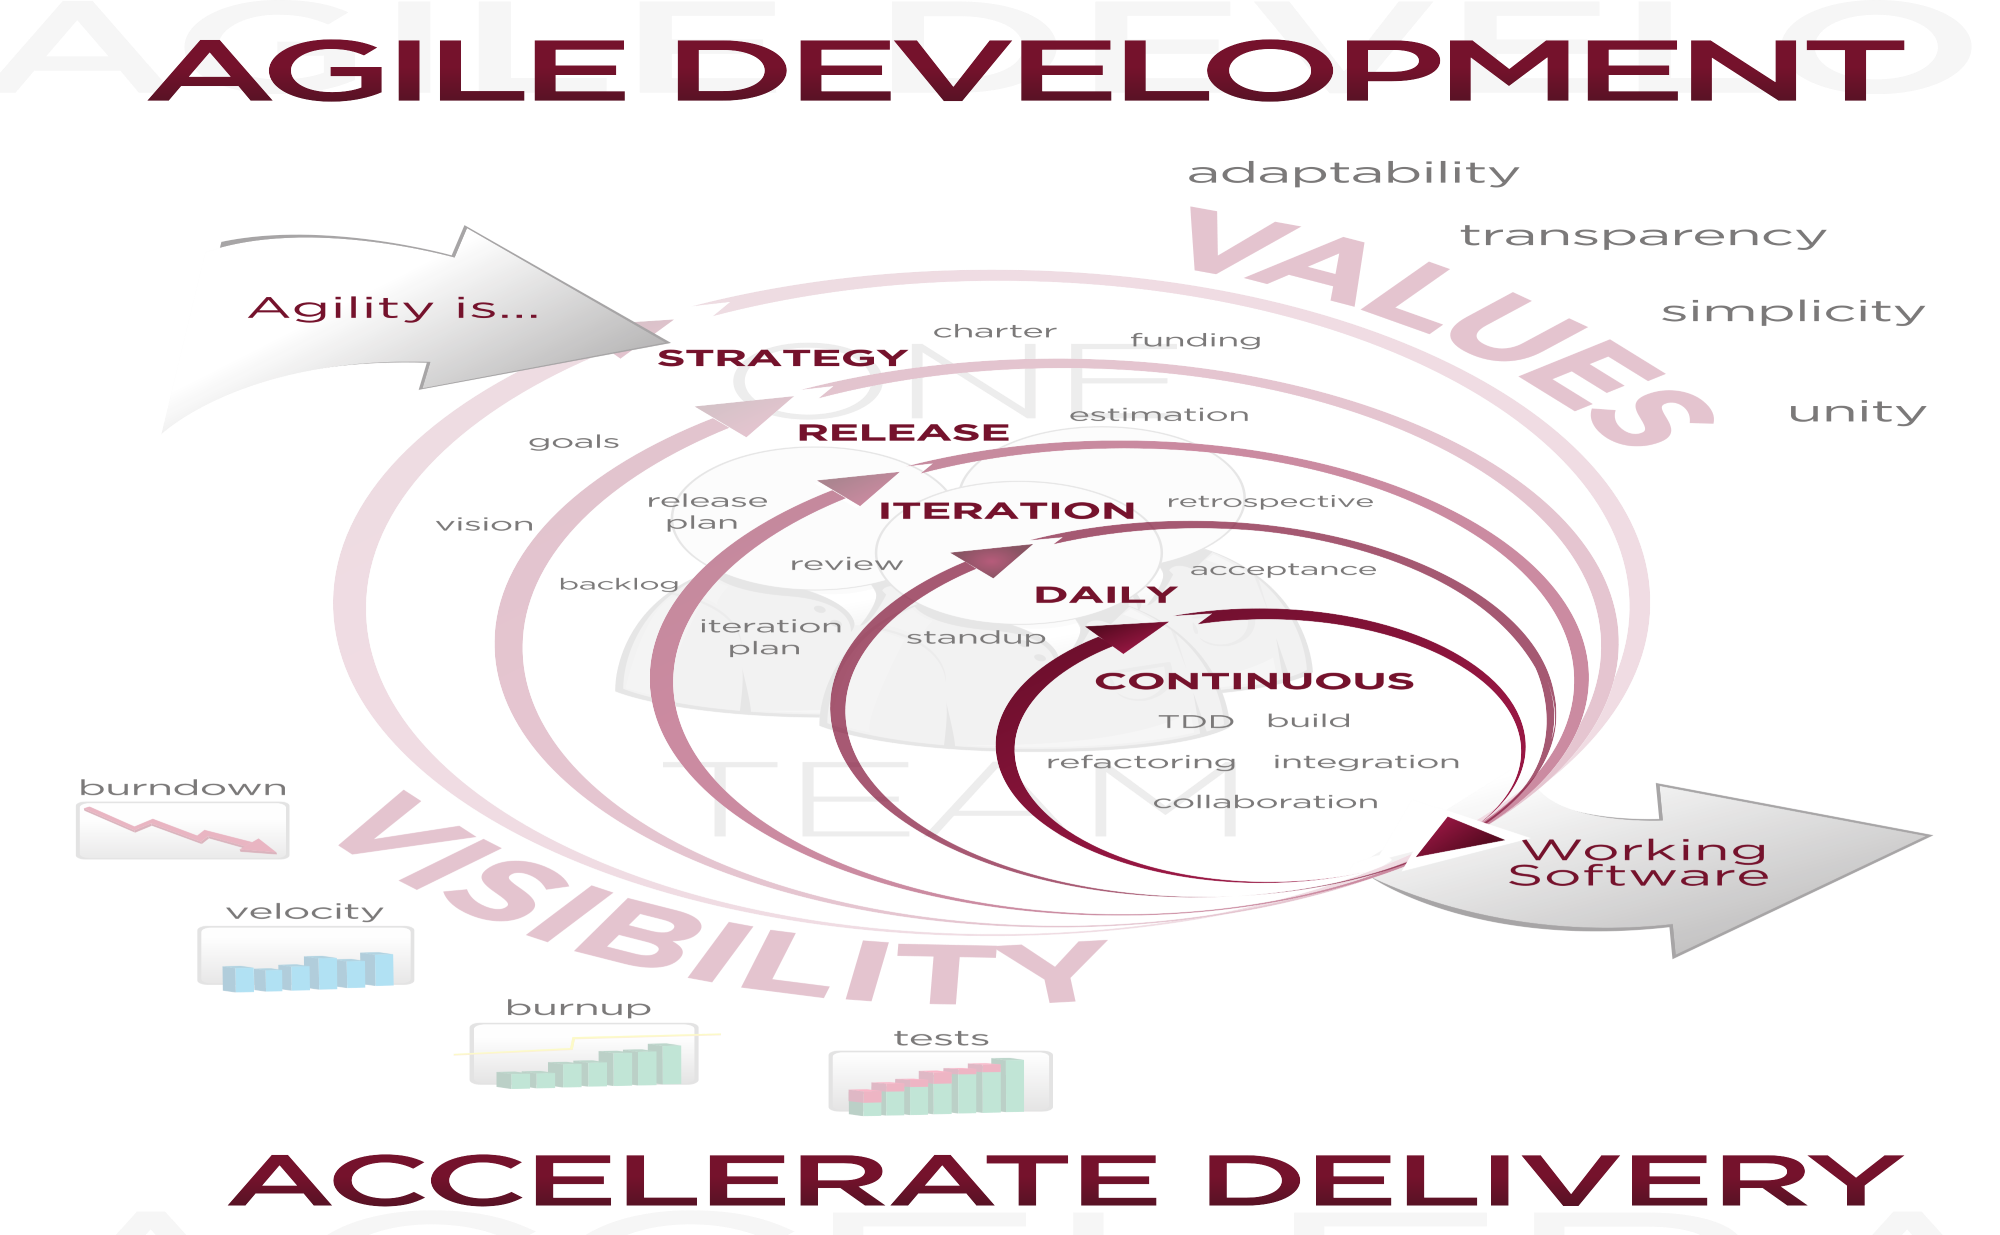
\includegraphics[width=0.8\textwidth, keepaspectratio=true]{agile_model}
\caption{Agile software development poster}
\end{figure}

The poster above represents the different iterations a team of developeres iterates through when using agile development meothodology.

\subsection{Scrum}
Scrum is a type of agile development, it has set intervalls(normally 2 to 4 weeks) for each milestone with each milestone containing about the same amount of work.

\begin{figure}[!htpb]
\label{logo}
\centering
	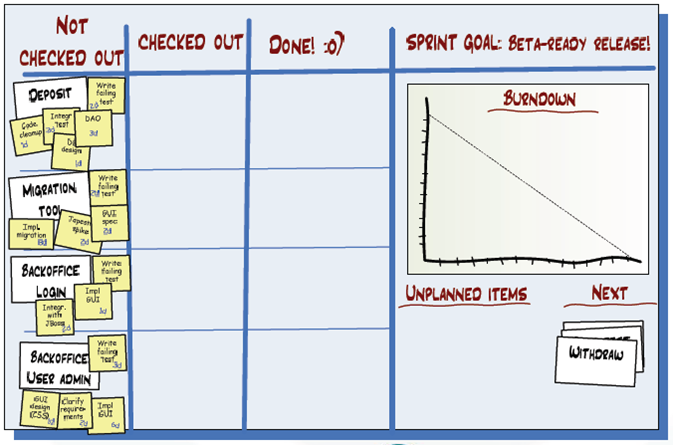
\includegraphics[width=0.8\textwidth]{scrumboard}
\caption{Example of scrum board}
\end{figure}

A scrumboard as shown above is used for each milestone to show which issues have been started on and who is working on which feature. The chart to the right is a burndown chart, stating how many hours the team has to work inorder to complete on time.